\section{Solución óptima}
\label{sec:solucion_optima}

De acuerdo con el diagrama de funciones presentado en la sección \ref{sec:CH03_FUNCIONES}, se elabora la matriz morfológica con las posibles opciones asociadas a cada función. A partir de esta matriz, se establecen conexiones entre funciones con el fin de estructurar tres alternativas de solución. Para ello, en el Anexo \ref{an:Anexo_G} se organiza la matriz por los dominios definidos en la sección \ref{sec:CH03_FUNCIONES}, lo que permite plantear de manera ordenada los conceptos de solución. En esa misma línea, el Anexo \ref{an:Anexo_W} reúne los tres conceptos obtenidos mediante la combinación de componentes de la matriz morfológica, incluyendo la descripción de sus elementos y dibujos del sistema en vista exterior e interior. Finalmente, la evaluación técnico-económica se realiza considerando dichos conceptos y, conforme a la metodología VDI 2221 \autocite{imagen_v}, los puntajes y pesos asignados a cada criterio se detallan en el Anexo \ref{an:Anexo_V}.

En la Figura~\ref{fig:solucion_ganadora} se presentan las vistas interna y externa del concepto seleccionado, correspondientes a la Figura~\ref{fig:solucion_ganadora_interna} y la Figura~\ref{fig:solucion_ganadora_externa}, respectivamente. Tras el análisis técnico-económico de las alternativas, documentado en el Anexo~\ref{an:Anexo_V}, se determinó como ganadora al concepto de solución 3. En las secciones siguientes se describe en mayor detalle cada subsistema que conforma el sistema \ac{HW} tomando como referencia el concepto elegido.
\begin{figure}[htbp]
    \centering
    \begin{subfigure}[b]{0.48\textwidth}
        \centering
        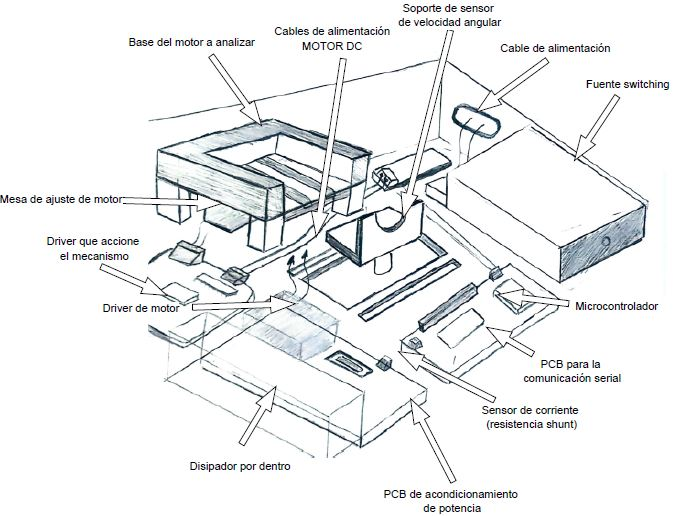
\includegraphics[width=\textwidth]{CHPTRS/CH03_DICON/Fig/CH03_FIG02_CoS/13_CoS_Solucion3porDentro.JPG}
        \caption{Vista interna de la solución óptima}
        \label{fig:solucion_ganadora_interna}
    \end{subfigure}
    \hfill
    \begin{subfigure}[b]{0.48\textwidth}
        \centering
        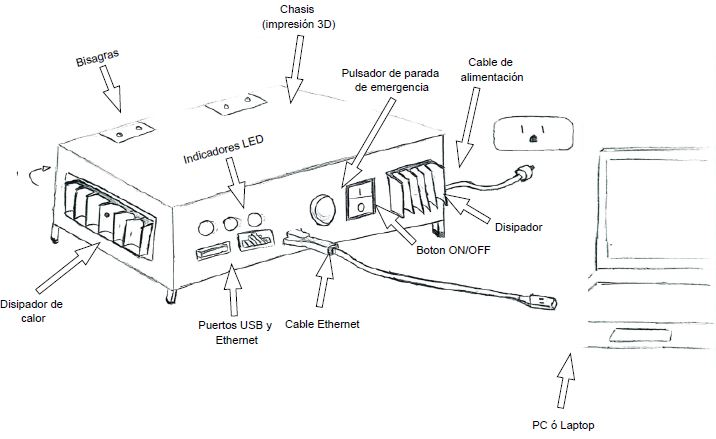
\includegraphics[width=\textwidth]{CHPTRS/CH03_DICON/Fig/CH03_FIG02_CoS/09_CoS_Solucion3porFuera.JPG}
        \caption{Vista externa de la solución óptima}
        \label{fig:solucion_ganadora_externa}
    \end{subfigure}

    \caption{Vistas interna y externa de la solución óptima seleccionada.}
    \label{fig:solucion_ganadora}
\end{figure}
    
Se comenzará definiendo la construcción del chasis, el cual deberá cumplir con las medidas limitadas indicadas en la sección \ref{sec:.lista de req}. Este chasis tendrá dimensiones que no excedan los 125x176 mm. Con base en estas dimensiones, se diseñará el chasis tomando en cuenta el tamaño de los componentes que irán por dentro y las \ac{PCB}s que se diseñen para el sistema. Cabe resaltar que la solución ganadora utiliza una fuente conmutada \textit{switching}. Estas fuentes, como tal, ya vienen con una carcasa que ocupa demasiado espacio si se mantiene dentro del sistema. Por lo tanto, se optará por usar únicamente la \ac{PCB} de esta fuente junto con los respectivos disipadores de calor, ya que la carcasa de la fuente \textit{switching} sirve principalmente para la disipación. 
Por otra parte, en cuanto al lugar donde se apoyará el motor, se mejorará la forma de ajuste, reemplazándolo por soportes diseñados específicamente para cada motor a analizar. En la Figura \ref{fig:dunker} se muestra un motor modelo Dunkermotor GR 42x40 \textcite{dunkermotoren}, al cual se le fabricaron dichos soportes para su análisis. Ahora bien, los agujeros, de la Figura  en la parte inferior estarán estandarizados, de forma que permitan la sujeción en la estructura ranurada donde se apoyará el motor. Si el motor resulta ser muy grande, se dejará un agujero en el chasis para evitar interferencias al momento de fijarlo.
    

\begin{figure}[H]
    \centering
    \begin{subfigure}[H]{0.4\textwidth}
        \centering
        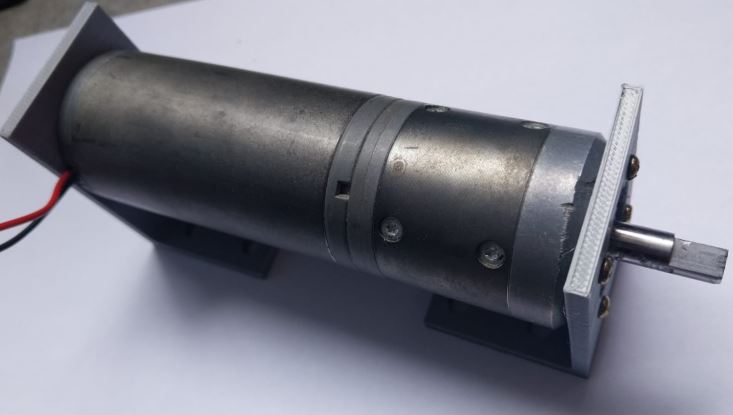
\includegraphics[width=\textwidth]{CHPTRS/CH03_DICON/Fig/CH03_FIG03_SolucionOptima/02a_SO_SoporteMotor.JPG}
       \caption{Prueba del acople diseñado para sujetar un motor de la marca Dunkermotor}
       \label{fig:dunker}
    \end{subfigure}
    \hfill
    \begin{subfigure}[H]{0.4\textwidth}
        \centering
        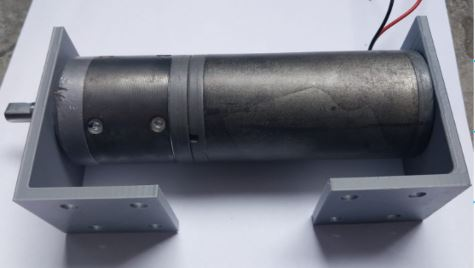
\includegraphics[width=\textwidth]{CHPTRS/CH03_DICON/Fig/CH03_FIG03_SolucionOptima/02b_SO_AgujerosDeSoporte.JPG}
       \caption{Agujeros estandarizados para estos soportes de motor}
       \label{fig:dunker}
    \end{subfigure}
    \caption{Pruebas de soportes impresos para un motor DC de la marca \autocite{dunkermotoren}}
    \label{fig:figura_con_subfiguras}
    \end{figure}
     Además, si el motor es muy pequeño, se optará por diseñar acoples como los que se muestran en la Figura \ref{fig:acople_pequeno}.
     \begin{figure}[H]
       \centering
       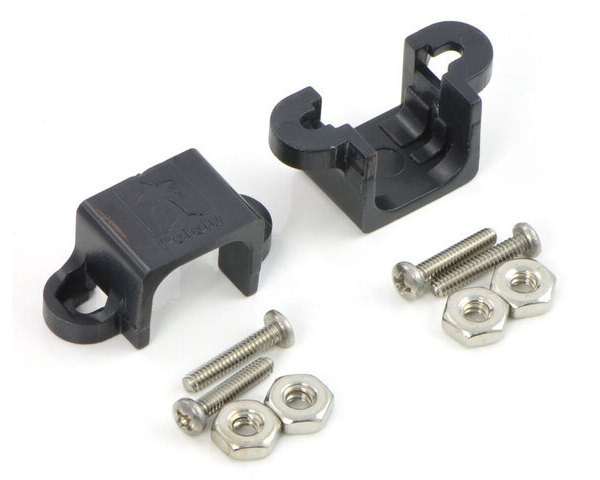
\includegraphics[width=0.3\textwidth]{CHPTRS/CH03_DICON/Fig/CH03_FIG03_SolucionOptima/03_SO_SoporteDeMotorPequeno.jpg}
       \caption{Acople para motores de diámetros reducidos, basados en los soportes de \textcite{pololu}}
       \label{fig:acople_pequeno}
    \end{figure}

    Para el diseño del acople del disco de imanes, se tomó de  inspiración como los mandriles y mordazas utilizados en máquinas de manufactura como tornos o taladros. Este enfoque permite que el disco sea adaptable a una amplia variedad de diámetros de ejes de motor, alcanzando hasta 15 mm. La fijación se logra mediante tornillos de sujeción ubicados en los costados, garantizando estabilidad durante las pruebas.
    Además, la inercia del disco será previamente conocida para restarla durante la estimación de parámetros, lo que permitirá determinar con mayor precisión la inercia real del motor analizado.
    De la empresa \textcite{pololu} se puede tomar  de inspiración que el disco donde estén los imánes sea similar a una acople universal ajustable como se muestra en la Figura \ref{fig:acople_universal}
    

    \begin{figure}[H]
    \centering
    \begin{subfigure}[H]{0.30\textwidth}
        \centering
        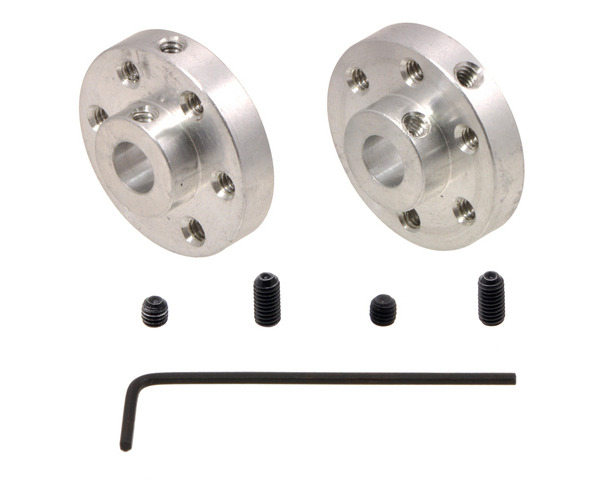
\includegraphics[width=\textwidth]{CHPTRS/CH03_DICON/Fig/CH03_FIG03_SolucionOptima/04a_SO_MotorPololu1.jpg}
       \caption{Elementos para el ajuste de la unión}
       \label{fig:dunker}
    \end{subfigure}
    \hfill
    \begin{subfigure}[H]{0.3\textwidth}
        \centering
        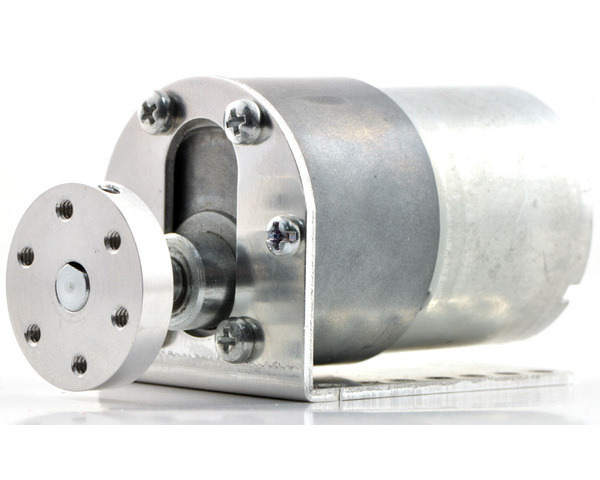
\includegraphics[width=\textwidth]{CHPTRS/CH03_DICON/Fig/CH03_FIG03_SolucionOptima/04b_SO_MotorPololu2.jpg}
       \caption{Motor de la empresa Pololu utilizando el acople universal}
       \label{fig:dunker}
    \end{subfigure}
    \caption{Acople universal brindado por la empresa Pololu}
    \caption*{Imágenes extraídas de la página oficial de \textcite{pololu}}
    \label{fig:acople_universal}
    \end{figure}
    
    Para la selección del \textit{encoder} magnético se optó por utilizar este sensor en lugar de uno óptico, debido a las ventajas que presenta. Mientras que los sensores ópticos son susceptibles al polvo y generan ruido en las mediciones, los sensores magnéticos ofrecen mayor precisión, siempre y cuando no se encuentren con alguna de interferencias, como los campos magnéticos generados por el propio motor \autocite{maxon_encoders}. La resolución del encoder magnético depende del número de imanes que tendrá el disco. Por ejemplo, un disco con 8 imanes genera 8 pulsos por vuelta (PPR). Sin embargo, aumentar la cantidad de imanes para mejorar la precisión implica una complicación, ya que incrementa la frecuencia de interrupciones que debe procesar el microcontrolador a elegir. Esto podría saturar su capacidad si no está diseñado para manejar altas frecuencias o si tiene otras tareas en ejecución.\\
   Para garantizar mediciones precisas, en la validación se corroborará si el sensado de velocidad debe realizarse directamente en el eje del motor o si sensar en el eje de salida del reductor no introduce distorsiones relevantes. A priori, medir en el eje del motor sería más preciso al evitar las tolerancias mecánicas de los engranajes del reductor; sin embargo, se verificará cuánto influye esta diferencia considerando la resolución del \textit{encoder} que se elegirá utilizar.
   
    \begin{figure}[H]
       \centering
       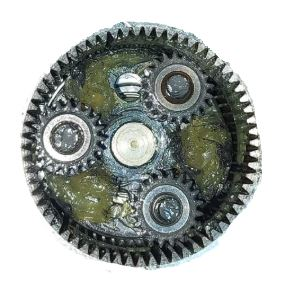
\includegraphics[width=0.35\textwidth]{CHPTRS/CH03_DICON/Fig/CH03_FIG03_SolucionOptima/05_SO_EngranajesPlanetario.JPG}
       \caption{Caja de engranajes planetarios luego de extraer la carcasa del reductor al motor modelo Dunkermotor GR 42x40 }
       \label{fig:planetario}
    \end{figure}
    
    % En la Figura \ref{fig:IMAGENES_XTRAS}, el sensado ocurre directamente en el eje del motor, incluso cuando se usa una caja reductora para la operación del motor.
    
    Para la fijación y calibración de la posición del \textit{encoder} se realizará mediante una estructura ajustable en dos ejes, inspirada en el módulo mostrado en la Figura \ref{fig:sist_cntrl}. Esta estructura permite calibrar la posición óptima de los sensores de efecto Hall en relación al disco con imanes. El proceso de calibración deberá ser realizado por el usuario y se estima que no tomará más de 5 minutos. Se diseñará para ser intuitivo y requerirá únicamente herramientas básicas como destornilladores y tornillos, facilitando su ajuste incluso para usuarios sin experiencia técnica avanzada.

    \begin{figure}[H]
    \centering
    \begin{subfigure}[H]{0.3\textwidth}
        \centering
        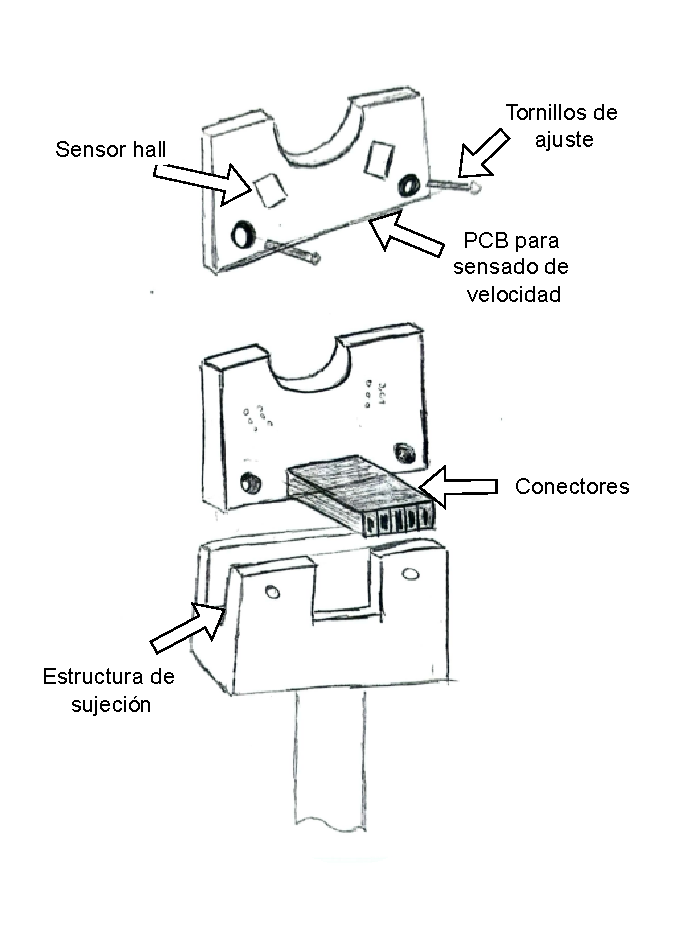
\includegraphics[width=\textwidth]{CHPTRS/CH03_DICON/Fig/CH03_FIG03_SolucionOptima/06a_SO_EncoderMagnetico.pdf}
       \caption{Bosquejo de la tarjeta de sensado, tomando como referencia la Figura \ref{fig:IMAGENES_XTRAS}}
       \label{fig:dunker}
    \end{subfigure}
    \hfill
    \begin{subfigure}[H]{0.3\textwidth}
        \centering
        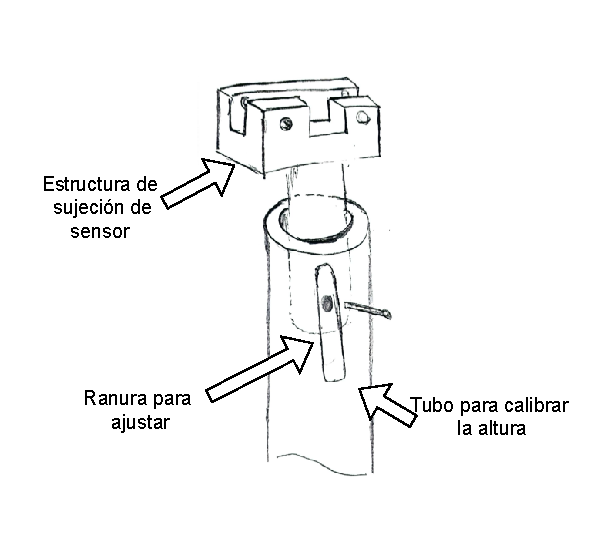
\includegraphics[width=\textwidth]{CHPTRS/CH03_DICON/Fig/CH03_FIG03_SolucionOptima/06b_SO_SoporteDeEncoder.pdf}
       \caption{Bosquejo de soporte de la placa de censado de velocidad}
       \label{fig:dunker}
    \end{subfigure}
    \caption{Bosquejo a mano alzada de las piezas que se utilizan para censar velocidad}
    \label{fig:sist_cntrl}
    \end{figure}
    Con todo lo mencionado, el usuario podrá calibrar por sí mismo tanto la posición del soporte del motor como la distancia del sensor de velocidad. Esta flexibilidad se ha implementado como una medida para adaptarse a la diversidad de motores con distintas geometrías, garantizando que las soluciones mecánicas sean lo más estandarizadas y versátiles posible.
    
    % A continuación, en la Figura \ref{fig:diagrama_flujo}, se presenta el diagrama de flujo de operaciones para el uso de la máquina estimadora.
    % \begin{figure}[b!]
    %    \centering
    %    \includegraphics[width=0.4\textwidth]{CH04_DICON/Fig_sol_optima/IMAGENES-Página-16.drawio.pdf}
    %    \caption{Diagrama de flujo de la máquina diseñada}
    %    \label{fig:diagrama_flujo}
    % \end{figure}

    % Como se observa, la lógica del \ac{SW} y \ac{HW} del sistema deberá estar diseñada para cumplir con todas estas funcionalidades. El usuario deberá permanecer atento ante posibles fallas, mientras que la solución desarrollada deberá incluir la electrónica necesaria para garantizar la automatización del proceso. Asimismo, la parte mecánica deberá asegurar la sujeción precisa y en todo momento de los sensores y las \ac{PCB}s diseñadas para la solución final.